\documentclass{article}
\usepackage{graphicx}
\usepackage[margin=1.5cm]{geometry}
\usepackage{amsmath}

\begin{document}

\title{Warm Up: Unit 1 Kinematics and Calculus Exercise}
\author{Prof. Jordan C. Hanson}
\maketitle

\section{Memory Bank}

\begin{enumerate}
\item The derivative, or slope, of a function $f(t) = a t^n + b$ is $f'(t) = a n t^{n-1}$.  For example, if $f(t) = \frac{1}{2} a t^2$, then the derivative is $f'(t) = a t$, because $n = 2$.  If $f(t) = at$, then $f'(t) = a$, because $n=1$.
\item $v(t) = a t + v_i$ ... Velocity of a system at a time $t$ is the acceleration ($a$) times time, plus initial velocity $v_i$.
\item $x(t) = \frac{1}{2}a t^2 + v_i t + x_i$ ... The position of a system at time $t$ is equal to one-half the acceleration times time squared, plus initial velocity times time, plus initial position.
\end{enumerate}

\section{Calculus Exercises}

\begin{enumerate}
\item Let $f(t) = 3 t + 2$.  Evalute the following:
\begin{itemize}
\item $f(-\frac{2}{3})$
\item $f'(t)$
\item $f'(-\frac{2}{3})$
\end{itemize}
\item Let $f(t) = \frac{3}{2} t^2 - \frac{3}{2}$.  Evalute the following:
\begin{itemize}
\item $f(1)$
\item $f'(t)$
\item $f'(1)$
\end{itemize}
\end{enumerate}

\section{Chapters 3.1 - 3.6}

\begin{enumerate}
\item The \textit{instantaneous velocity} is the derivative or slope of position versus time.
\begin{figure}[hb]
\centering
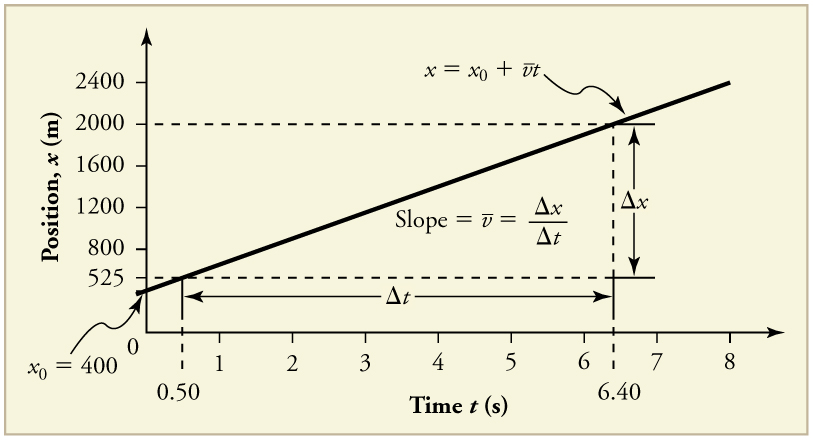
\includegraphics[width=0.33\textwidth]{figures/slope.jpeg}
\end{figure}
(a) What is the instantaneous velocity at $t_0$? (b) Is the average velocity between $t_1$ and $t_6$ greater than, less than, or equal to the instantaneous velocity at $t_0$?
\item If $x(t) = \frac{3}{2} t^2 + 10$ meters, what is $v(t)$?  What is $v(1)$?  \textit{Assume time is measured in seconds.}
\end{enumerate}

\end{document}
